\documentclass[10pt,pdf]{beamer}
\usetheme{Goettingen}
\title{Latex Practice}
\author{Vadim Khanin}
\institute{HSE}
\date{ July 2021}
\definecolor{col0}{RGB}{0, 255, 68}
\setbeamercolor{itemize item}{fg=green}    
\setbeamercolor{enumerate item}{fg=red}    
\begin{document}

\section{Title Page}
\frame{\titlepage}

\begin{center}
\section{Content}
\begin{frame}
\frametitle{Content}
\tableofcontents
\end{frame}
\end{center}

\begin{frame}
\frametitle{Intro}
\section{Intro}
Slides of the following presentation are remade from my presentation for coursework.
\end{frame}

\section{Tasks And Solutions}
\begin{frame}
\frametitle{Subtasks and methods od their implementation}
\begin{columns}[T,onlytextwidth]
    \begin{column}{0.3\textwidth}
        \begin{enumerate}
        \item Split videos into frames 
        \item Detect and extract the skin on the image
        \item Extract dominant color on the image 
        \end{enumerate}
    \end{column}
    \begin{column}{0.1\textwidth}
    \bigskip    
    \LARGE
    \textcolor{blue}{$\rightarrow$\\}
    \vspace{0.5cm}
    \textcolor{blue}{$\rightarrow$\\}
    \vspace{0.6cm}
    \textcolor{blue}{$\rightarrow$\\}
    \normalsize
    \end{column}
    \begin{column}{0.4\textwidth}
    \begin{itemize}
        \item def video\underline{ }to\underline{ }frames(path)
        \vspace{0.1cm}
        \item def extract\underline{ }skin(image)
        \vspace{0.4cm}
        \item def extract\underline{ }dominant\underline{ }color\\(image,\\number\underline{ }of\underline{ }colors=1\\,hasThresholding=False)
    \end{itemize}
    \end{column}
\end{columns}
\end{frame}


\section{Example of extracting skin color}
\begin{frame}
\frametitle{Extracting skin}
Here is an example of extracing dominant color from the image.
\begin{columns}
    \begin{column}{0.4\textwidth}
    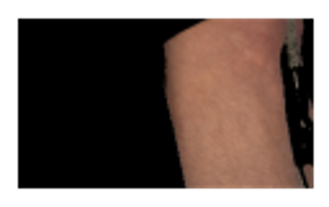
\includegraphics[width=\textwidth,scale=1]{pres1.png}
    \end{column}
    \begin{column}{0.3\textwidth}
    \LARGE
    \textcolor{blue}{$\rightarrow\rightarrow\rightarrow\rightarrow\rightarrow$\\}
    \normalsize
    \end{column}
    \begin{column}{0.35\textwidth}
    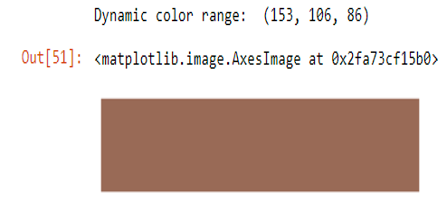
\includegraphics[width=\textwidth]{pres2.png}
    \end{column}
\end{columns}
\end{frame}

\section{Conclusion}
\begin{frame}
\frametitle{Conclusion and prospects for further work.}
\begin{itemize}
    \item[\textcolor{magenta}{\textbullet}] \textcolor{magenta}{The average differences between rgb values of dominant skin colors are lower for healthy people than for people, ill with phlebological diseases. 
}
    \item[\textcolor{red}{\textbullet}] \textcolor{red}{The maximum deviation of rgb values of dominant skin colors is lower for healthy people than for people, ill with phlebological diseases.}
    
    \item[\textcolor{col0}{\textbullet}] \textcolor{col0}{As a result, the average values of the real values were obtained for groups of patients and healthy people. This research shows, that these values differ among groups. Hence the algorithm may be useful in early noninvasive diagnosis of venous diseases.}

\end{itemize}
\end{frame}

\end{document}